\section{Detección de la pelota}\label{chapter:deteccion}


La recopilación de información del medio ambiente, para detectar la posición de la pelota, se realiz\'o por medio de la cámara Raspberry Pi dado que una cámara otorga mayor información y más precisa. 

El procesamiento de las imagenes es realizado por la mini computadora Raspberry Pi sobre la cual ha sido instalado el sistema operativo Raspian.

TightVNC se utilizó para la visualización y control de la interfaz gráfica de Raspbian en la Raspberry Pi desde un computador remoto, pues es conveniente poder observar lo que el robot percibe para llevar un control y una supervisión de su comportamiento.

Con ayuda de la librería OpenCv, en C++, se filtra y procesa la imagen para obtener la posición de la pelota. Esta librería también ofrece funciones para capturar la imagen de algunos tipos de cámara, sin embargo con el módulo de cámara de la Raspberry Pi no funciona. Por ello se ha utilizado la librería raspicam cv robidouille que permite obtener la imagen en una estructura de datos que puede ser utilizado por las funciones de OpenCv. 

Para encontrar la ubicación de la pelota en un momento dado y de forma autónoma se ha decidido aplicar detección por ‘blobs’, o reconocimiento de regiones, esta técnica consiste en filtrar la imagen por color, por ello es importante que el de la pelota no se repita en el ambiente y así poder obtener la posición de la pelota dentro de la imagen.

La imagen es captada en el modelo de color RGB y se transforma al HSV. Luego se aplica la función inRange de OpenCv para obtener una imagen en blanco y negro, en donde se identifica con blanco la zona con el color de la pelota y el resto de la imagen en negro. 

Para disminuir el ruido y los posibles elementos aislados que pueda tener la imagen con la que se está trabajando se han aplicado los filtros o transformaciones de morfología en apertura y morfología en clausura de la librería Opencv, basadas en las operaciones básicas de dilatación y erosión. La morfología en apertura es una transformación que consiste en aplicar la operación de erosión seguido de la operación de dilatación REF. La morfología de clausura es una transformación que aplica la dilatación seguido de la erosión.

De esta forma se logró ubicar la pelota con la cámara Raspberry Pi con buenos resultados en la mayoría de los casos. 
 
\subsection{Comunicación Arbotix - Raspberry (ROS)}

La Raspberry Pi procesa la información de la cámara y la Arbotix controla los actuadores. Para coordinar los movimientos del robot según la posición de la pelota se estableció una forma de comunicación entre ambas tarjetas. 

Se ha establecido la Arbotix como servidor de peticiones y a la Raspberry Pi como cliente. Dentro de la Raspberry Pi se ejecuta el proceso de decidir qué acción debe tomar el robot. Una vez determinada la acción se envía la petición a la Arbotix para que esta la ejecute. Este proceso es bidireccional y síncrono, es decir, la Raspberry envía la petición y se bloquea hasta que la Arbotix retorne la respuesta de su culminación.  

Para la implementación de la comunicación se ha usado ROS con su versión Hydro y se ha utilizado la interfaz de comunicación basada en servicios que no es más que un método de comunicación basado en el paradigma de resquest / reply con el concepto de maestro esclavo. REF

\subsection{Estrategia - Visión - Acciones}

El hecho de  que la cámara tenga dos grados de libertad para moverse es una gran ventaja, ya que se puede obtener un mayor rango de visión. Debupa puede mirar hacia la derecha o izquierda sin tener que mover sus piernas, también puede mirar hacia abajo para verificar que la pelota esté en sus pies, para patear, o hacia arriba para ubicar la pelota a mayor distancia.

La estrategia para poder llegar a la pelota consiste en mover la posición de la cámara hasta encontrar la pelota, en caso de encontrarla, dependiendo de su ubicación dentro de la imagen y la posición de la cámara se toma una acción diferente, en caso de no encontrarla el robot gira con los pies para cambiar su orientación física e iniciar nuevamente el movimiento de la cámara para hallar la pelota. Cuando se tiene la pelota en una posición cercana a los pies se realiza la acción de patear. 

En la siguiente sección se explicará la manera en la que se dividen las regiones en una imagen para determinar la acción a tomar y el orden en el que se mueve la cámara.

\subsection{Discretización del ambiente}


Debupa debe tomar una acción diferente dependiendo de la posición de la cámara y de la pelota en la imagen. Sin embargo esto genera una gran cantidad de estados, por lo cual se ha decidido discretizarlos de la siguiente manera:  

La cámara tiene 6 (2x3) posibles posiciones. La visión horizontal abarca 3 cuadros, aproximadamente 160 grados, por razones de la estructura del robot no se le ha podido agregar un rango más grande. La visión vertical abarca 2 cuadros, llega a captar la imagen desde sus pies hasta más de 2 metros hacia adelante.

Desde cada posición de la cámara se obtiene una imagen. Las imagenes de la cámara en posición central, y en posicion central inferior son las más importantes y prioritarias, pues si la pelota se detecta en ellas significa que el robot está cerca de poder patearla. Estas dos imagenes se dividen en subregiones, para tener mayor precisión en las acciones que Debupa deba tomar. Una representación sencilla de la discretizacion del ambiente se puede apreciar en la figura ~\ref{fig:divisionCam}. El área de pateo son las regiones 15 y 16. Por ejemplo, en el cuadro del central inferior, cuando la pelota se encuentra del lado derecho de la pantalla (region 13 o 17) el robot debe girar a la derecha para situarse de frente a la pelota.

Las imágenes capturadas desde cada posición de la cámara se solapan para evitar perder de vista a la pelota. 

Las acciones específicas a tomar según el estado en que se encuentre la pelota se realizan por medio de lo aprendido en el entrenamiento realizado con apredizaje por reforzamiento. Los detalles de este aprendizaje se describen en la seccion 3.4.
%A continuación se especifica la acción a tomar en cada region: 
 
%Girar a la Izquierda: Debupa debe girar a la izquierda cuando la pelota se encuentre en alguna de las siguientes regiones: 1, 4, 10, 5, 11, 14.

%Girar a la Derecha: debe girar a la derecha cuando la pelota se ubique en alguna de las siguientes regiones: 7, 13, 17, 3, 9, 18. 

%Caminar hacia adelante: cuando la pelota se ubique en alguna de las siguientes regiones: 12, 6, 2.

%Patear con la pierna izquierda: cuando la pelota se encuentre en la región 15.

%Patear con la pierna derecha: cuando la pelota se encuentre en la región 16.

\begin{figure}[hbtp]

\centering
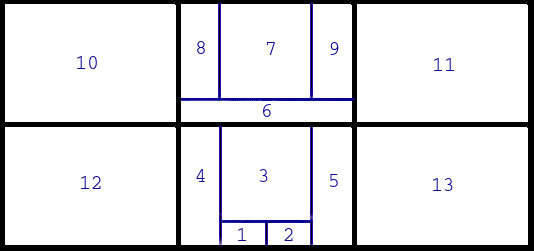
\includegraphics[scale=0.5]{imagenes/Regiones.jpg}
\caption{Campo de visión del robot con el número de cada región. Cada cuadro blanco demarcado con líneas negras representa la posición de la cámara. La región de pateo de la pelota se encuentra en los cuadros 15 y 16 }
\label{divisionCam}
\end{figure}
